\documentclass[12pt,a4paper,titlepage,headinclude,bibtotoc]{scrartcl}

%---- Allgemeine Layout Einstellungen ------------------------------------------

% Für Kopf und Fußzeilen, siehe auch KOMA-Skript Doku
\usepackage[komastyle]{scrpage2}
\pagestyle{plain}
\setheadsepline{0.5pt}[\color{black}]
\automark[section]{chapter}


%Einstellungen für Figuren- und Tabellenbeschriftungen
\setkomafont{captionlabel}{\sffamily\bfseries}
\setcapindent{0em}


%---- Weitere Pakete -----------------------------------------------------------
% Die Pakete sind alle in der TeX Live Distribution enthalten. Wichtige Adressen
% www.ctan.org, www.dante.de

% Sprachunterstützung
\usepackage[ngerman]{babel}

% Benutzung von Umlauten direkt im Text
% entweder "latin1" oder "utf8"
\usepackage[utf8]{inputenc}

% Pakete mit Mathesymbolen und zur Beseitigung von Schwächen der Mathe-Umgebung
\usepackage{latexsym,exscale,stmaryrd,amssymb,amsmath}


\usepackage[nointegrals]{wasysym}
\usepackage{eurosym}

% Anderes Literaturverzeichnisformat
%\usepackage[square,sort&compress]{natbib}
\usepackage{hyperref}
% Für Farbe
\usepackage{color}
\usepackage{graphicx}
\usepackage{wrapfig}
\usepackage{subfigure}

% Caption neben Abbildung
\usepackage{sidecap}

% Befehl für "Entspricht"-Zeichen
\newcommand{\corresponds}{\ensuremath{\mathrel{\widehat{=}}}}
% Befehl für Errorfunction
\newcommand{\erf}[1]{\text{ erf}\ensuremath{\left( #1 \right)}}

%Fußnoten zwingend auf diese Seite setzen
\interfootnotelinepenalty=1000

%Für chemische Formeln (von www.dante.de)
%% Anpassung an LaTeX(2e) von Bernd Raichle
\makeatletter
\DeclareRobustCommand{\chemical}[1]{%
  {\(\m@th
   \edef\resetfontdimens{\noexpand\)%
       \fontdimen16\textfont2=\the\fontdimen16\textfont2
       \fontdimen17\textfont2=\the\fontdimen17\textfont2\relax}%
   \fontdimen16\textfont2=2.7pt \fontdimen17\textfont2=2.7pt
   \mathrm{#1}%
   \resetfontdimens}}
\makeatother

%Honecker-Kasten mit $$\shadowbox{$xxxx$}$$
\usepackage{fancybox}

%SI-Package
\usepackage{siunitx}

%keine Einrückung, wenn Latex doppelte Leerzeile
\parindent0pt

%Bibliography \bibliography{literatur} und \cite{gerthsen}
%\usepackage{cite}
\usepackage{babelbib}
\selectbiblanguage{ngerman}

\begin{document}

\begin{titlepage}
\centering
\textsc{\Large Praktikum zur Einführung in die physikalische Chemie,\\[1.5ex] Universität Göttingen}

\vspace*{0.5cm}

\rule{\textwidth}{1pt}\\[0.5cm]
{\huge \bfseries
  V5: Leitfähigkeit\\[1.5ex]
  wässriger Elektrolyte}\\[0.5cm]
\rule{\textwidth}{1pt}

\vspace*{0.5cm}


\begin{Large}
\begin{tabular}{ll}
Durchführende: &  Alea Tokita, Julia Stachowiak\\
Assistentin: & Annemarie Kehl\\
 Versuchsdatum: & 01.02.2016\\
 Datum der ersten Abgabe: & 08.02.2016\\

\end{tabular}
\end{Large}

\vspace*{1cm}
\begin{large}
\begin{table} [h]
\centering 
\begin{tabular}{p{3cm}|p{5cm}p{5cm}}
& Messwerte & Literaturwerte\footnotemark\\
\hline
Essigsäure & &\\
 $K_{\mathrm{S}}$  bei $25^\circ\text{C}$ & $2,5 \cdot 10^{-5} \pm 1,5 \cdot 10^{-7}$& $1,738 \cdot 10^{-5}$\\
$\Lambda^0\, [\mathrm{S} \cdot \mathrm{m^2} \cdot \mathrm{mol^{-1}}]$ & $ 0,030\, \pm 0,012 $& 0,03905\\
\hline
Kaliumchlorid & &\\
$\Lambda^0\, [\mathrm{S} \cdot \mathrm{m^2} \cdot \mathrm{mol^{-1}}]$ & 0,015 $\pm$ 0,000025 & 0,01503\\
\end{tabular}
\end{table}
\end{large}

%\begin{Large}
%\fbox{
%  \begin{minipage}[t][9cm][t]{10cm} 
%\textbf{Messwerte:}\\
%Kaliumchlorid: \\
%$\Lambda^0 = 0,015\, \mathrm{S} \cdot \mathrm{m^2} \cdot \mathrm{mol^{-1}}$\\
%Essigsäure:\\
% $K_{\mathrm{S}} = 2,5 \cdot 10^{-5} \pm 1,5 \cdot 10^{-7}$\\
%$\Lambda^0 = 0,03\, \mathrm{S} \cdot \mathrm{m^2} \cdot \mathrm{mol^{-1}}$\\ 
%\textbf{Literaturwerte:}\\
%Kaliumchlorid: \\
%$\Lambda^0 = 0,01503\, \mathrm{S} \cdot \mathrm{m^2} \cdot \mathrm{mol^{-1}}$\protect\footnotemark\\
%Essigsäure:\\
%$\Lambda^0 = 0,03905 \mathrm{S} \cdot \mathrm{m^2} \cdot \mathrm{mol^{-1}}$\protect\footnotemark\\
%$K_{\mathrm{S}} = 1,8 \cdot 10^{-5}$\protect\footnotemark\\  
 % \end{minipage}
%}
%\end{Large}

\end{titlepage}

\tableofcontents

\newpage

\section{Theorie}
Ziel des Versuchs ist es, die Grenzleitfähigkeiten eines starken und eines schwachen Elektrolyten zu bestimmen. Dies erfolgt über Leitfähigkeitsmessungen verschieden konzentrierter Lösungen des Elektrolyten.
\subsection{Elektrolyt}
Unter einem wässrigen Elektrolyten $\mathrm{M}_{v+}\mathrm{A_{v-}}$ versteht man einen Stoff, welcher im Wasser in positive und negative Ionen (Kationen und Anionen) dissoziiert. Es wird dabei zwischen schwachen und starken Elektrolyten unterschieden. Ein starker Elektrolyt dissoziiert vollständig in Anionen und Kationen, wobei $v_+$ und $v_-$ die stöchiometrischen Koeffizienten der Dissoziationsreaktion sind und die Ionen verschiedene Ladungszahlen $z_+\mathrm{bzw} z_-$ tragen.\\\\
Ein schwacher Elektrolyt dissoziiert nur teilweise in Lösung, der Dissoziationsgrad $\alpha $ gibt den Bruchteil der eingesetzten Stoffmenge $n_0$ der dissozierten Moleküle an. Dabei liegen $v_{\pm } \cdot \alpha \cdot n_0$ Mol an postiven und negativen Ionen vor, da gilt:
\begin{align}
\alpha = \dfrac{n_0 - n_u}{n_0}
\end{align} 
Wobei $n_u$ die Stoffmenge der undissoziierten Teilchen angibt.
\subsection{Leitfähigkeit}
Ein Maß für die Leitfähigkeit einer Lösung und demzufolge auch des darin enthaltenen Elektrolyten, ist ihr elektrischer Widerstand $R$. Nach dem Ohmschen Gesetzt gilt folgende Abhängikeit von der elektrischen Spannung $U$ under der Stromstärke $I$:
\begin{align}
\dfrac{U}{I} = R = \mathrm{const}.
\end{align}
$R$ ist dabei abhängig von den geometrischen Dimensionen des Stromleiters. Im einfachsten Fall eines metallischen Leiters der Länge $l$ und Querschnittsfläche $A$, ist der Widerstand umso stärker je größer $A$ und je kleiner $l$ ist. Demnach ist der Widerstand durch die Abmessungen sowie andererseits durch eine Materialkonstante, der spezifische Wiederstand $\rho $ gegeben:
\begin{align}
R = \rho \dfrac{l}{A} \quad \quad  [R]=  \mathrm{m}
\end{align} 
%\Ohm !!!
Da ein Material den Strom umso besser leitet, je geringer sein Widerstand ist, verwendet man den Leitwert $L$, um seine charakteristischen Eigenschaften zu beschreiben. Die Erfassung der geometrischen Abmessungen der Messzelle ist aufgrund der komplizierten Ionenwanderung sehr schwierig, daher wird die Proportionalitätsfaktor $Z$ zwischen $R$ und $\rho$ eingeführt. Des weiteren wird der reziproke Wert des spezifischen Widerstands als $\kappa$ bezeichnet:
\begin{align}
L = \dfrac{1}{R} = \dfrac{1}{\rho } \dfrac{A}{l} = \dfrac{\kappa }{Z}
\end{align} 
Da die Leitfähigkeit von der Einwaagekonzentration abhängig ist, definiert man die molare Leitfähigkeit $\Lambda$ einer Elektrolytlösung mit der Einwaagekonzentration $c^*$:
\begin{align}
\Lambda = \dfrac{\kappa}{c^*}
\end{align}

\subsection{Kohlrausches Quadratwurzelgesetz, Grenzleitfähigkeit}
Ionen haben eine unterschiedliche Beweglichkeit und unterschiedliche Ladungen, daher tragen sie in unterschiedlicher Weise zur Gesamtleitfähigkeit bei. Daher ist die molare Leitfähigkeit wiederum Konzentrationsabhängig, dies gilt selbst bei vollständiger Dissoziation, da sich Ionen in ihrer Bewegung gegenseitig Beeinflussen.\\
Eine wichtige Bezugsgröße ist die molare Grenzleitfähigkeit $\Lambda^0$, welche der bei unendlicher Verdünnung gemessenen molaren Leitfähigkeit entspricht. Sie kann aus einer Extrapolation $ \lim \limits_{c \rightarrow 0 } \Lambda = \Lambda ^0$ bestimmt werden und setzt sich additiv aus den Anteilen einzelner Ionensorten zusammen.\\\\
Das nach Kohlrausch benannte Quadratwurzelgesetz beschreibt die Konzentrationsabhängigkeit der molaren Leitfähigkeit:
\begin{align}
\Lambda = \Lambda ^0 - \kappa \cdot \sqrt{c}
\end{align}
\subsection{Unvollständige Dissoziation, Ostwaldsches Verdünnungsgesetzt}
Die Konzentrationsabhängigkeit der molaren Leitfähigkeit ist bei schwachen Elektrolyten wesentlich stärker. Da sie nicht vollständig dissoziieren gilt das Kohlrausche Quadratwuzelgesetz nicht. Die Leitfähigkeit ist stark durch die Gleichgewichtskonzentration bestimmt.\\\\
Stellt man das Massenwirkungsgesetzt für die Dissoziation eines schwachen Elektrolyten auf und setzt für die Konzentration des Elektrolyten deren Verhältnis der Einwaagekonzentration $c^*$ zum Dissoziationsgrad ein, erhält man folgenden Ausdruck:
\begin{align}
K_\mathrm{S} = \dfrac{\alpha ^2}{1-\alpha } \cdot \dfrac{c^*}{c^0}
\end{align}
Zur Leitfähigkeit tragen nur die Ionen des dissoziierten Elektrolyten bei. Bei sehr kleinen Einwagekonzentrationen ($c^* \rightarrow 0$) dissoziieren schwache Elektrolyte vollständig, jedoch ist dann auch die Ionenkonzentration sehr klein. Auch bei höheren Einwaagekonzentrationen ist die Ionenkonzentration aufgrund des niedrigen Dissoziationsgrades die Ionenkonzentration klein. Dementsprechend kann man in guter Näherung annehmen, dass die Leitfähigkeit proportional zur Zahl der dissoziierten Moleküle und damit proportional zum Dissoziationsgrad $\alpha$ ist. Somit gilt näherungweise für die molare Leitfähigkeit:
\begin{align}
\lambda = \alpha \cdot \Lambda ^0 
\end{align}    
Setzt man dies Beziehung in Gleichung ein, erhält man das Ostwaldsche Verdünnungsgesetzt:
\begin{align}
K_\mathrm{S} = \dfrac{c^* \cdot \Lambda ^2}{c^0 \cdot \Lambda ^0 \cdot (\Lambda ^0 - \Lambda)}
\end{align} 
 Aus der Auftragung von $\dfrac{1}{\Lambda}$ gegen $c^* \cdot \Lambda$ lässt sich die Säurekonstante und die Grenzleitfähigkeit ermitteln, entsprechend der Gleichung umgestellt:
\begin{align}
\dfrac{1}{\Lambda} = \dfrac{1}{\Lambda ^0} * \dfrac{c^* \cdot \Lambda }{K_\mathrm{S} \cdot (\Lambda ^0)^2 \cdot c^\circ}
\end{align}

\newpage
\section{Versuchsaufbau}
\begin{figure} [h!]
\begin{center}
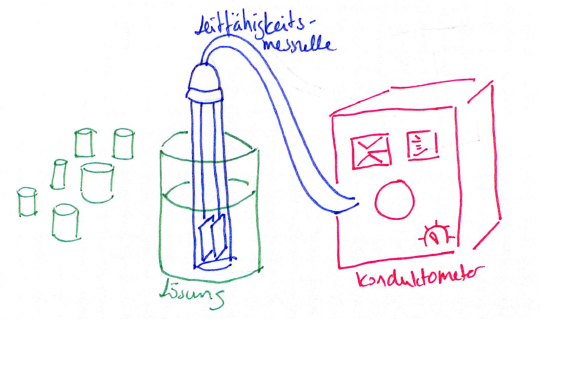
\includegraphics[scale=1]{Versuchsaufbau.png} \end{center}
\caption {Versuchsaufbau}
\end{figure}

Gemessen wird der elektrische Leitwert $L$ der Elektrolytlösung in der elektrochemischen Zelle eines Konduktometers. Dies erfolgt im genaueren mithilfe einer Wheatstone-Brückenschaltung. Die verwendeten Zellen zeigen bei Abgleich der Messbrücke auf den Zeigerauschlag null direkt den Leitert $L$ an. Auch die Zellkonstante $Z$ ist bereits gegeben.
\section{Versuchdurchführung}
Da die Konzentrationsabhängigkeit der molaren Leitfähigkeit von Kaliumchlorid- und Essigsäurelösungen bestimmt werden sollen, werden zunächst Essigsäure- und Kaliumchloridlösungen der Konzentration $0,1 {~}\mathrm{M}$, $0,01{~}\mathrm{M}$ und $0,001{~}\mathrm{M}$ hergestellt. Dies erfolgt über das Verdünnen von $0,1{~}\mathrm{M}$ Lösungen der Elektrolyten.\\\\
Bei den Messungen wird mit der Messung der Eigenleitfähigkeit von destillierten Wasser, welches zum Verdünnen benutzt wurde, begonnen, um eine Abschätzung des Einflusses der Eigenleitfähigkeit des Wassers auf die Messergebnisse zu ermöglichen. Anschließend wird bei den Messungen der Elektrolytlösungen die Lösung der geringsten Konzentration zuerst gemessen. Die Leifähigkeit der Lösungen wird mindestens fünfmal gemessen und zu jeder Messung die Temperatur der Lösung notiert. Beim Messen muss darauf geachtet werden, dass Stellrad am Konduktometer nur langsam und vorsichtig zu bewegen.\\\\
Vor der Messung werden Becherglas, Tauchelektrode und das Thermometer mehrfach mit destilliertem Wassern und anschließend mit der zu messenden Lösung gespült. Zur Messung wird das Becherglas so weit mit der Messlösung gefüllt, dass dass die Tauchglocke der Elektroden vollständig bedeckt ist und zur vollständigen Benetzung vorsichtig mit der Elektrode gerührt. Zwischen den Messungen wird die Elektrode gründlich mit destilliertem Wasser gespült.



\newpage

\section{Auswertung}

Aus den Messungen werden die Mittelwerte des Leitwertes $L$ bestimmt und die Eigenleitfähigkeit des Wassers davon abgezogen. Mit der Zellkonstante $Z$ der Leitfähigkeits-Messzelle wird die spezifische Leitfähigkeit $\kappa$ für jede Lösung errechnet:\\

\begin{equation}
\kappa = \frac{Z}{R} = Z \cdot L
\end{equation}

Daraus ergibt sich die molare Leitfähigkeit $\Lambda$ der Lösungen:\\

\begin{equation}
\Lambda = \frac{\kappa}{c^*}
\end{equation}

Für die Auftragungen wird die molare Leitfähigkeit bei der gemessenen Temperatur auf die Leitfähigkeit bei $25^\circ\text{C}$ umgerechnet, der Koeffizient $m$ ist für die beiden Lösungen unterschiedlich:\\

\begin{equation}
\Lambda (25^\circ\text{C}) = \Lambda(\Omega) \cdot [1+ m \cdot (25- (\Omega/^\circ\text{C}))]
\end{equation}\\

{\centering
$m_{\mathrm{KCl}} = 2,31 \cdot 10^{-2}$ für $0,1\, \mathrm{M} \ge c_s \ge 0,001\, \mathrm{M}$\\
$m_{\mathrm{HAc}} = 1,44 \cdot 10^{-2}$ für $0,1\, \mathrm{M} \ge c_s \ge 0,001\, \mathrm{M}$\\}



\subsection{Bestimmung von $\Lambda^0$ und $K_{\mathrm{S}}$ für Essigsäure}

Für den schwachen Elektrolyten kann das Ostwaldsche Verdünnungsgesetz umgeformt werden:\\

\begin{equation}
\frac{1}{\Lambda} = \frac{1}{\Lambda^0} + \frac{c^* \cdot \Lambda}{K_{\mathrm{S}} \cdot (\Lambda^0)^2 \cdot c^0}
\end{equation}

Aufgetragen wird $\frac{1}{\Lambda}$ gegen $\frac{c^* \cdot \Lambda}{c^0}$.
Der reziproke Wert für die Grenzleitfähigkeit $\Lambda^0$ ergibt somit durch Extrapolation des Graphen als Schnittpunkt mit der Ordinate.\\
Als Steigung $m$ bleibt  $m = \frac{1}{K_{\mathrm{S}} \cdot (\Lambda^0)^2 }$.\\
Die Säurekonstante $K_{\mathrm{S}}$ errechnet sich damit folgendermaßen:\\

\begin{equation}
K_{\mathrm{S}} = \frac{1}{m \cdot (\Lambda^0)^2}
\end{equation}

Nach Abziehen der Eigenleitfähigkeit des Wassers und Umformen ergeben sich folgende Werte für die Auftragung:\\

\begin{table} [h]
\centering 
\begin{tabular}{|p{4cm}||p{4cm}|p{4cm}|}
\hline
& $\frac{1}{\Lambda(25^\circ\text{C})}$ in $\frac{\mathrm{mol}}{\mathrm{S} \cdot \mathrm{m^2}}$ & $\frac{c^*}{c^0} \cdot \Lambda(25^\circ\text{C})$ in $\frac{\mathrm{S} \cdot \mathrm{m^2}}{\mathrm{mol}}$\\
\hline
0,1 M & 1918 & $5,213 \cdot 10^{-5}$  \\
\hline
0,01 M & 614,0 & $1,629 \cdot 10^{-5}$  \\
\hline
0,001 M & 210,8 & $4,473 \cdot 10^{-5}$ \\
\hline
\end{tabular}
\end{table}

Daraus ergibt sich:\\

$K_{\mathrm{S}} = 2,5 \cdot 10^{-5}$\\
$\Lambda^0 = 0,03\, \mathrm{S} \cdot \mathrm{m^2} \cdot \mathrm{mol^{-1}}$\\





\subsection{Bestimmung von $\Lambda^0$ für Kaliumchlorid}

Für den starken Elektrolyten Kaliumchlorid wird das Kohlrausche Quadratwurzelgesetz $\Lambda$ gegen $\sqrt{c}$ aufgetragen:\\

\begin{equation}
\Lambda = \Lambda^0 - k \cdot \sqrt{c}
\end{equation}

$\Lambda^0$ ergibt sich ebenfalls aus Extrapolation als Schnittpunkt mit der Ordinate.

Für die Auftragung ergeben sich als Werte:\\


\begin{table} [h]
\centering 
\begin{tabular}{|p{4cm}||p{4cm}|p{4cm}|}
\hline
& $\Lambda(25^\circ\text{C})$ in $\frac{\mathrm{S} \cdot \mathrm{m^2}}{\mathrm{mol}}$ & $\sqrt{c}$ in $\mathrm{mol^{\frac{1}{2}}} \cdot \mathrm{l^{- \frac{1}{2}}}$\\
\hline
0,1 M & 0,01239 & 0,3162 \\
\hline
0,01 M & 0,01407 & 0,1000 \\
\hline
0,001 M & 0,01439 & 0,03162 \\
\hline
\end{tabular}
\end{table}

Für $\Lambda^0$ ergibt sich somit:\\
$\Lambda^0 = 0,015\, \mathrm{S} \cdot \mathrm{m^2} \cdot \mathrm{mol^{-1}}$\\

\newpage 

\section{Fehlerrechnung}

\subsection{absolute Fehler}
Die absoluten Fehler bzw. Messungenauigkeiten der Geräte betragen:\\

\begin{table} [h]
\centering 
\begin{tabular}{p{4cm}p{4cm}}
$\Delta$ Temperatur & $= 0,1^\circ\text{C}$ \\
$\Delta$ Kolben &$= 1$ mL   \\
$\Delta$ Pipette &  $=0,1$ mL \\
\end{tabular}
\end{table}

Der Fehler der Temperatur bzw. des Termometers ist vernachlässigbar klein und nur der Vollständigkeit halber aufgeführt. Er wird in der weiteren Fehlerrechnung vernachlässigt.\\
 Der Fehler der Einwaagekonzentration $c*$ ergibt sich somit:\\
 
 


\subsection{Fehlerrechnung}
Zuerst wird die absolute Standartabweichung der Leitwerte nach folgender Formel bestimmt:\\

\begin{equation}
s_{\mathrm{N}} = \sqrt{\frac{1}{N-1} \sum_{i=1}^{N}(x_i -\bar{x})}
\end{equation} 

Da es sich um sehr wenige Werte handelt (jeweils 5), muss die Standartabweichung noch mit dem Student'schen t-Faktor multipliziert werden, um den Fehler für $\bar{L}$ zu erhalten:\\

\begin{equation}
\Delta \bar{L} = t_N \cdot \bar{s}_N
\end{equation}

Für $95,5 \%$ Konfidenz und 5 Messwerte beträgt dieser 2,8\protect\footnotemark

\footnotetext{Götz, Eckold: \emph{Grundbegriffe der Fehleranalyse bei praktischen Messungen}, Institut für physikalische Chemie, Uni Göttingen, \textbf{2015}.}


Somit ergeben sich folgende Fehler für $\bar{L}$:

\begin{table} [h]
\centering 
\begin{tabular}{|p{4cm}||p{2cm}|p{2cm}|p{2cm}|}
\hline
& 0,1 M & 0,01 M & 0,001 M \\
\hline
Essigsäure & & & \\
$\bar{L}$ in $\mu \mathrm{S}$ &746 & 235 & 69,9\\
$s_N$ in $\mu \mathrm{S}$ & 5,5 & 1,9 & 1,1 \\
$\Delta L$ in $\mu \mathrm{S}$ & 15& 5,4& 3,1\\
\hline
Kaliumchlorid & & &\\
$\bar{L}$ in m $\mathrm{S}$& 17,6 & 1,98 & 0,204\\
$s_N$ in m $\mathrm{S}$ & 0,17 & 0,017 & 0,0025\\
$\Delta L$ in m $\mathrm{S}$ & 0,47& 0,047& 0,0070\\
\hline
\end{tabular}
\end{table}

\newpage
\subsection{Fehlerfortpflanzung für $\Lambda$}
$\Lambda$ wird in den Rechnungen weiterverwandt und aufgetragen, sodass eine Fehlerfortpflanzung nach Gauß durchgeführt werden muss. Die Formel dafür lautet:\\

\begin{equation}
\Delta f = \sqrt{\sum_i \left(\frac{\delta f}{\delta x_i}\right)^2_j \cdot \Delta x_i^2}
\end{equation}

Aus $\kappa = Z \cdot L$ und $c^* =\frac{n}{V}$ ergibt sich:\\

\begin{equation}
\Lambda = \frac{\kappa}{c^*}= \frac{Z \cdot L \cdot V}{n}
\end{equation}

Der Fehler für das Volumen setzt sich hierbei additiv aus denabsoluten Fehlern für Kolben und Pipette zusammen:\\

\begin{equation}
\Delta V = \Delta \mathrm{Kolben} + \Delta \mathrm{Pipette} = 1,1 \cdot 10^{-3} L
\end{equation}

%Eingesetzt in die Formel für die Umrechnung von $\Lambda$ auf 25 Grad ergibt sich eine absolute Formel, auf die die Fehlerrechnung angewandt werden kann:\\

%\begin{equation}
%\Lambda(25^\circ\text{C}) = \left(\frac{Z\cdot L \cdot V}{n}\right) \cdot [1+ m \cdot (25-(\Omega/^\circ\text{C}))]
%\end{equation}

%AB hier neu!!!!

\begin{equation}
\Delta \Lambda = \sqrt{\left(\frac{Z \cdot V}{n}\right)^2 \cdot {\Delta L}^2 + \left(\frac{Z \cdot L}{n}\right)^2 \cdot \Delta V^2}
\end{equation}

Daraus ergeben sich folgende Fehler für $\Delta \Lambda$, welche als Fehlerbalken in die Auftragungen eingetragen werden.\\

\begin{table} [h]
\centering 
\begin{tabular}{|p{7cm}||p{2cm}|p{2cm}|p{2cm}|}
\hline
& 0,1 M & 0,01 M & 0,001 M \\
\hline
$\Delta \Lambda$ Essigsäure $[\mathrm{S \cdot m^{2} \cdot mol^{-1}}]$ & $1,2 \cdot 10^{-6}$ & $3,5 \cdot 10^{-5}$& $2,1 \cdot 10^{-4}$ \\
\hline
$\Delta \Lambda$ Kaliumchlorid $[\mathrm{S \cdot m^{2} \cdot mol^{-1}}]$ &$3,1 \cdot 10^{-4}$ & $3,1 \cdot 10^{-4}$ & $4,9 \cdot 10^{-5}$ \\
\hline
\end{tabular}
\end{table}





\newpage

\subsection{Fehler für $\Lambda^0$ und $K_{\mathrm{S}}$ aus der Auftragung}

Durch die eingezeichneten Grenzgeraden kann aus der maximalen und minimalen Steigung der absolute Fehler für $\Lambda^0$ bestimmt werden:\\


\begin{equation}
\frac{1}{K_{\mathrm{S}\,\mathrm{min}}} =\left( \frac{17600-400}{0,048-0,009} \right)= 44\cdot 10^4
\end{equation}

\begin{equation}
\frac{1}{K_{\mathrm{S}\,\mathrm{max}}}\,=\,\left(\frac{17700-230}{0,05-0,004}\right)\,=\, 38 \cdot 10^4
\end{equation}


\begin{equation}
K_{\mathrm{S}\,\mathrm{min}} = 2,3 \cdot 10^{-6}
\end{equation}

\begin{equation}
K_{\mathrm{S}\,\mathrm{max}} = 2,6 \cdot 10^{-6}
\end{equation}


Somit ergibt sich der absolute Fehler von $K_{\mathrm{S}}$:\\

\begin{equation}
\Delta K_{\mathrm{S}} = \frac{K_{\mathrm{S}\,\mathrm{max}} - K_{\mathrm{S}\,\mathrm{min}}}{2} = 1,5 \cdot 10^{-7}
\end{equation}


$\Lambda^0$ wurde in beiden Fällen durch Extrapolation des Graphen als Schnittpunkt mit der Ordinate bestimmt. Analog ergibt sich auch der absolute Fehler aus dem maximalen bzw. minimalen Schnittpunkt mit der Achse. \\
\\
Essigsäure:\\

\begin{equation}
\left(\frac{1}{\Lambda^0}\right)_\mathrm{max} = 90\, \mathrm{mol \cdot m^{-2} \cdot S^{-1}}
\end{equation}

\begin{equation}
\left(\frac{1}{\Lambda^0}\right)_\mathrm{min} = 20\, \mathrm{mol \cdot m^{-2} \cdot S^{-1}}
\end{equation}

\begin{equation}
\Delta \Lambda^0 = \Lambda^0 - \frac{2}{(\frac{1}{\Lambda^0})_\mathrm{max} + (\frac{1}{\Lambda^0})_\mathrm{min}} = 0,012\, \mathrm{S \cdot m^2 \cdot mol^{-1}}
\end{equation}

Analog ergibt sich auch $\Delta \Lambda^0$ für Kaliumchlorid:\\

\begin{equation}
\Lambda^0_\mathrm{max} = 0,0015\, \mathrm{S \cdot m^{2} \cdot mol^{-1}} 
\end{equation}

\begin{equation}
\Lambda^0_\mathrm{min} = 0,00145\, \mathrm{S \cdot m^{2} \cdot mol^{-1}} 
\end{equation}

\begin{equation}
\Delta \Lambda^0 = \Lambda^0 - \frac{\Lambda^0_\mathrm{max} \cdot \Lambda^0_\mathrm{min}}{2} = 0,000025 \, \mathrm{S \cdot m^{2} \cdot mol^{-1} = 2,5 \cdot 10^{-5}\, \mathrm{S \cdot m^{2} \cdot mol^{-1}}} 
\end{equation}





\subsection{Diskussion systematischer Fehler}

Systematische Fehler bei der Versuchsdurchführung ergeben sich hauptsächlich aus Ableseungenauigkeiten der Geräte und Fehler beim Verdünnen. Die 0,1 M Lösung wurde nicht selbst hergestellt, sodass der Fehler hier nicht bekannt ist.\\

In der Rechnung vernachlässigt wurde die Messungenauigkeit des Thermometers, der Fehler ist demnach wahrscheinlich größer als errechnet. Um diese Fehlerquelle besser zu berücksichtigen, müsste die Fehlerfortpflanzung in die Umrechnungsformel der Temperatur mit eingebaut werden.\\

Die Eigendissoziation des Wassers wurde berücksichtigt.\\

Am fehleranfälligsten bzw. ungenausten ist die Bestimmung der Größen durch die Auftragung. Pro Elektrolyt stehen am Schluss nur drei Messwerte zur Verfügung, von denen sich nur zwei richtig verbinden lassen. Das zeichnen der Verbindungsgerade erfolgt nach Augenmaß und kann sehr verschieden ausfallen. Dadurch kann auch der Schnittpunkt mit der Ordinate und somit der Wert für $\Lambda^0$ sehr unterschiedlich ausfallen. Eine zu kleine Steigung würde einen Schnittpunkt bei einem zu großen Wert mit der Ordinate bedeuten und somit ein zu kleines $\Lambda^0$ für Essigsäure und zu großes $\Lambda^0$ für Kaliumchlorid. Diese Ungenauigkeit wurde in der Fehlerfortpflanzung und der grafischen Bestimmung der absoluten Fehler nicht berücksichtigt, sodass die Fehler der Größen tatsächlich deutlich größer sein werden als die in der Fehlerrechnung errechneten Fehler.\\
Formal ergibt sich die Bestimmung der Grenzleitfähigkeit aus dem Schnittpunkt mit der Ordinate (siehe Formel 15, 16), ist allerdings nur eine Näherung, da unendliche Verdünnung einer sehr kleinen Konzentration entspricht und nicht $c=0$. Der Wert müsste also aus einem Punkt kurz vor dem Schittpunkt bestimmt werden. Aus einem größeren Wert ergäbe sich eine kleinere Grenzleitfähigkeit für Essigsäure und größere Grenzleitfähigkeit für Kaliumchlorid.\\
Da die Genauigkeit der Auftragung zu klein ist, als dass dies eine Rolle spielen könnte, ist dieser Punkt nur der Vollständigkeit halber aufgeführt.\\


Außerdem ist das Gerät möglicherweise fehlerhaft und zeigt einen falschen Wert an.\\




\newpage 

\section{Diskussion}
\subsection{Vergleich mit Literaturwerten}

Es ergeben sich folgende Werte:\\

\begin{table} [h]
\centering 
\begin{tabular}{p{3cm}|p{5cm}p{5cm}}
& Messwerte & Literaturwerte\footnotemark\\
\hline
Essigsäure & &\\
 $K_{\mathrm{S}}$  bei $25^\circ\text{C}$ & $2,5 \cdot 10^{-5} \pm 1,5 \cdot 10^{-7}$& $1,738 \cdot 10^{-5}$\\
$\Lambda^0\, [\mathrm{S} \cdot \mathrm{m^2} \cdot \mathrm{mol^{-1}}]$ & $ 0,030\, \pm 0,012 $& 0,03905\\
\hline
Kaliumchlorid & &\\
$\Lambda^0\, [\mathrm{S} \cdot \mathrm{m^2} \cdot \mathrm{mol^{-1}}]$ & 0,015 $\pm$ 0,000025 & 0,01503\\
\end{tabular}
\end{table}

\footnotetext{$http://www.uni-saarland.de/fak8/kazmaier/PDF_files/GV/GVF_Pkscarbo.pdf,\, abgerufen\,am\, 07.02.16.$}


\subsection{Diskussion}

Auffällig ist eine große Abweichung der Werte vom Literaturwert, die durch die Fehlergrenzen nicht mit einbegriffen wird. Mit einer Abweichung von 1 $\%$ der obersten Fehlergrenze vom Literaturwert liegt die Grenzleitfähigkeit von Kaliumchlorid sehr nah am Literaturwert. \\
Der Literaturwert der Grenzleitfähigkeit von Essigsäure wird durch die Fehlergrenzen mit eingeschlossen; für $K_\mathrm{S}$ ist der Fehler allerdings wieder zu klein.\\

In dem Versuch wird mit sehr vielen verschiedenen fehlerbehafteten Größen gerechnet (besonders beim Verdünnen der Lösungen), wodurch sich für die einzelnen Werte unterschiedlich große Fehlerbalken ergeben. Die grafische Bestimmung der Fehler ist schwierig, da nur wenig Messwerte vorhanden sind. \\

Die größten Fehlerquellen liegen demnach bei der Auswertung. Zur Verbesserung könnten die Leitfähigkeiten von noch schwächer verdünnten Lösungen gemessen werden, um die grafische Extrapolation zu vereinfachen.  \\

Fehler bzw. Ungenauigkeiten bei der Messung entstanden vor allem durch die Handhabung des Konduktometers. Durch das Springen der Skala um verschiedene Potenzen wurde das Ablesen der Werte sehr unübersichtlich und anfällig für Potenzfehler. Zwischenzeitiges Abspülen der Leitfähigkeits- Messzelle gestaltete sich außerdem als schwierig. \\

Letzendlich ergibt sich bei Essigsäure eine zu kleine Grenzleitfähigkeit, die von einer zu kleinen Konzentration kommen muss oder von einem fehlerhaften Messergebnis des Gerätes. Dadurch, dass $K_\mathrm{S}$ letzendlich mit dem reziproken Wert der Steigung berechnet wird, ergibt sich ein zu großer $K_\mathrm{S}$- Wert verglichen mit dem Literaturwert. \\
Die Abweichung der Grenzleitfähigkeit von Kaliumchlorid kann aufgrund der zu wenigen signifikanten Stellen nicht eindeutig bestimmt werden. Die Fehlergrenzen sind allerdings zu klein, was entweder von zu kleinen bestimmten Fehlern kommt systematischen Fehlern bei der Durchführung kommt. \\


\newpage

\section{Literaturverzeichnis}
\begin{flushleft}
1 \quad Gerd Wedler: \emph{Lehrbuch der physikalischen Chemie}, 5. Aufl., WILEY-VCH Verlag GmbH Co. KGaA, Weinheim, \textbf{2004}.\\
\vspace{0,5 cm}
2\quad Götz, Eckold: \emph{Sriptum zur Einführung in die physikalische Chemie}, Institut für physikalische Chemie, Uni Göttingen, \textbf{2015}.\\
\vspace{0,5 cm}
3 \quad \emph{Skriptum für das Praktikum zur Einführung in die Physikalische Chemie}, Institut für physikalische Chemie, Uni Göttingen, \textbf{2015}.\\
\end{flushleft}



\end{document}



